\subsubsection{Pixy (CMUcam5)}

Eine vielversprechende Möglichkeit zur Erkennung des Korbes ist der Bildsensor Pixy. Pixy kombiniert einen Bildsensor mit einem optimierten Prozessor und schickt das Resultat der Bildanalyse an einen Controller (z.B. Raspberry Pi). Dadurch muss der Controller nicht die grossen Bilddaten von einem Bildsensor berechnen, sondern kann seine Kapazitäten für andere Aufgaben einsetzten.

Um die Fähigkeiten von Pixy zu testen wurde ein Versuch durchgeführt. Bei normalen Tageslicht (bedeckter Himmel) wurde versucht den schwarzen Abfalleimer vor einer
weissen Wand einzulernen. Dabei stellte sich heraus das der Algorithmus von Pixy die Farbsättigung zur
Erkennung der Objekte verwendet. Der Abfalleimer ist schwarz und wird deshalb nicht von Pixy erkannt. Ein
farbiges Objekt, wie z.B. ein Tennisball wird sehr zuverlässig und schnell erkannt. Abbildung \ref{fig:pixy_objekt} zeigt wie Pixy einen
Leuchtstift erkennt. Der gesamte Einlernprozess hat gerade einmal 5 Minuten in Anspruch genommen.

\begin{figure}[h!]
	\centering
	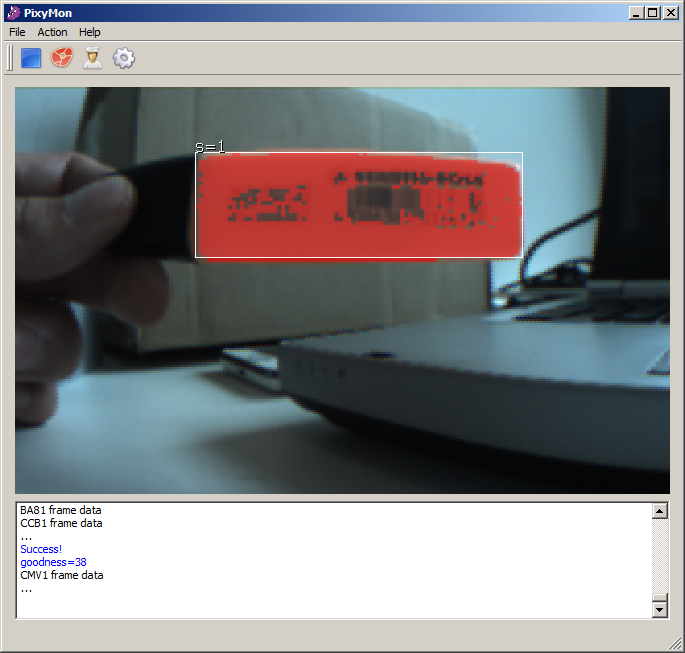
\includegraphics[width=0.7\linewidth]{../../fig/pixy_objekt}
	\caption{Pixy erkennt einen Leuchtstift}
	\label{fig:pixy_objekt}
\end{figure}

Damit Pixy den Korb erkennt, müsste der gesamte Algorithmus umgeschrieben werden. Da dies jedoch ein immensen Aufwand bedeutet wird Pixy nicht zur Erkennung des Korbes eingesetzt.